\chapter{Simple Machines}

As mentioned earlier, physicists define work as the force applied times the 
distance over which it is applied. For example, if you push your car 100 meters 
with a force of 17 newtons, you have done 1700 joules of work.

Humans have long needed to move heavy objects, so many centuries ago, we 
developed simple machines to reduce the amount of force necessary to perform 
such tasks. These include:

\begin{itemize}
    \item Levers
    \item Pulleys
    \item Inclined planes (ramps)
    \item Screws
    \item Gears
    \item Hydraulics
    \item Wedges
\end{itemize}

\includegraphics[width=\textwidth]{simplemachines.png}

While these machines can reduce the force needed, they do not change the total 
amount of work that must be done. For instance, if the force is reduced by a 
factor of three, the distance over which the force must be applied increases by 
the same factor.

The term \textit{mechanical advantage} refers to the increase in force achieved 
by using these machines.

\section{Mechanical Advantage}

As indicated above, mechanical advantage is the ratio between the force output 
by the machine and the force the user puts into the machine:
$$ MA = \frac{F_{out}}{F_{in}}$$

Since the input force is \textit{applied} to the simple machine, sometimes the 
input force is called an applied force and abbreviated as $F_a$. For example, 
you only need to apply a relatively little force to your car's brakes in order 
for the hydraulic braking system to apply enough force to your tires to stop 
them spinning (we'll examine this further below). 

\subsection{What does it mean to work hard?}
Humans use simple machines to ``make work easier", but what does this mean in a 
physics sense? Does using a machine actually decrease the amount of work the 
user has to do? When we say a task is easier, we usually mean \textit{we have to 
apply less force}. You might say that it is ``less work" to push something up a 
shallow incline than up a steep incline. But does the person pushing \textit{
actually do less work} (in a physics sense), or does that work simply require 
a smaller force? We'll answer this question by examining the physics of incline 
planes below, and the results will be true for all simple machines. 

\section{Inclined Planes}

Inclined planes, or ramps, allow you to roll or slide objects to a higher 
level. Steeper ramps require less mechanical advantage. For instance, it is much 
easier to roll a ball up a wheelchair ramp than a skateboard ramp.

\includegraphics[width=\textwidth]{rampcomparison.png}

Assuming the incline has a constant steepness, the mechanical advantage is 
equal to the ratio of the length of the inclined plane to the height it rises. 
%note to self: show why this is true or have students derive eqn in exercise -Max

If friction is neglected, the force required to push a weight up the inclined 
plane is given by:

\[
F_A = \frac{V}{L} F_g
\]
%FIXME ADD A diagram may be helpful here, locating v and l - Arjan
%how's the diagram below? -Max
% also explain why v and l is the inverse of mechanical advantage
% state that L is the hypotenuse formed by the tringle
where \( F_A \) is the applied force, \( L \) is the length of the inclined plane, \( V \) is the vertical rise, and \( F_g \) is the gravitational force acting on the mass.

\begin{center}
	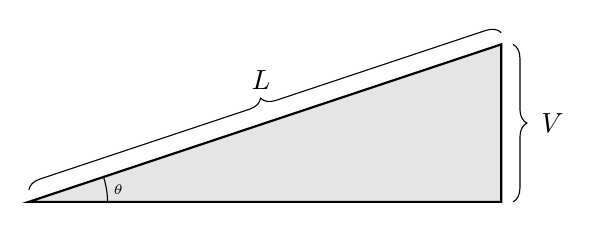
\begin{tikzpicture}
	   \draw[thick, black, fill=gray!20] (0,0) -- (6, 0) -- (6, 2) -- cycle;
          \draw[black] (1, 0) arc (0:18:1) 
          	node[font=\tiny, right, yshift = -0.15cm] {$\theta$};
          \draw[decorate, decoration = {brace, amplitude=5pt}] 
          	(0, 0.15) -- (6, 2.15);
          \node[] at (2.95, 1.55) {$L$};
          \draw[decorate, decoration = {brace, amplitude=5pt, mirror}] 
          	(6.15, 0) -- (6.15, 2);
          \node[] at (6.65, 1) {$V$};
	\end{tikzpicture}
\end{center}

(We will discuss sine function later, but in case you're familiar with it, note that:

\[
\frac{V}{L} = \sin{\theta}
\]

where \( \theta \) is the angle between the inclined plane and the horizontal surface.)

Let's compare the force needed and work done when pushing a load up a ramp 
versus just lifting it vertically. Consider a family on moving day: there's a 
hand trolley loaded with 200 N (about 45 pounds) of boxes. If the bed of the 
moving truck is 1.5 m high, how much work would it take to lift the boxes 
straight up into the truck? What about with a ramp? 

First, let's look at how much force and work is needed if you were to lift the 
entire 200 N load straight up into the air. You'd need to apply 200 N of force 
upwards for a distance of 1.5 m:
$$W = F \cdot d = \left( 200 \text{ N} \right) \left( 1.5 \text{ m} \right) = 300 \text{ J}$$

So, without a ramp, you would have to apply 200 N and do 300 J of work. Suppose 
your moving truck comes with a ramp that has an incline of 15 degrees:

\begin{center}
	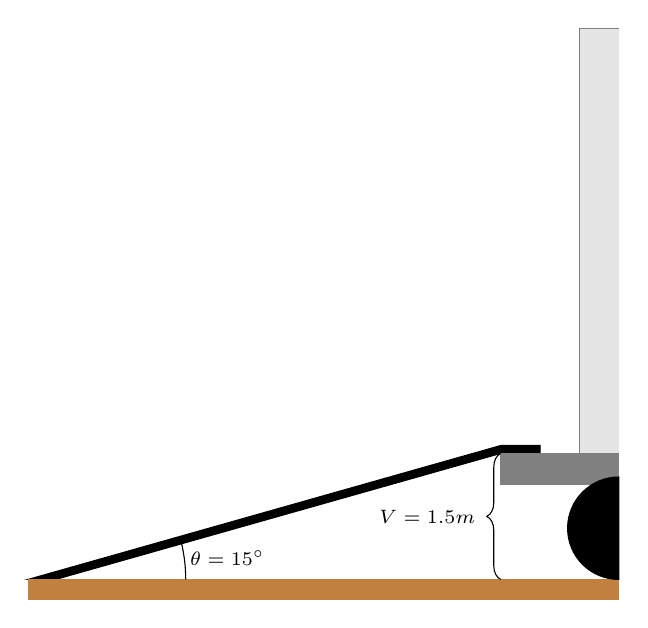
\begin{tikzpicture}
            \draw[black, fill=black] (0,0) -- (6, 1.7) -- (6.5, 1.7) -- 
            	(6.5, 1.6) -- (6, 1.6) -- (0.35, 0) -- cycle; 
	    	\draw[gray, fill=gray] (6, 1.2) rectangle (7.5, 1.6);
            \draw[brown, fill=brown] (0,-0.25) rectangle (7.5, 0);
            \draw[black, fill=black] (7.5, 1.3) arc (90:270:0.65) -- cycle;
            \draw[gray, fill=gray!20] (7.5, 1.6) -- (7, 1.6) -- (7, 7) -- (7.5, 7);
            \draw[black] (2, 0) arc (0:15:2) 
            	node[right, yshift = -0.25cm, font = \scriptsize] 
            	{
            	$\theta = 15^{\circ}$
            	};
            \draw[decorate, decoration = {brace, amplitude=5pt, mirror}] 
            (6, 1.6) -- (6, 0) 
            node[left, yshift = 0.8cm, xshift = -0.2cm, font = \scriptsize] 
            {
            $V=1.5\text{ m}$
            };
	\end{tikzpicture}
\end{center}

Since $\sin{ \left( \theta \right) } = V/L$, we know that $L = V / \sin{ \left( 
\theta \right) }$. You can use a calculator or search engine to find that the 
sine of $15^{\circ} \approx 0.26$. Therefore, the length of the ramp is 
approximately 5.8 meters. How much force does it take to move the load of boxes 
up the ramp? Intuitively, we know it is less force. We can use a 
\newterm{free body diagram} to determine the minimum force needed to push the 
box up the ramp. \index{free body diagram}(A free body diagram is a simplified 
model showing all the forces acting on an object. You'll learn to create and 
use your own free body diagrams in a later chapter. For now, just follow along.)

Before you push it, there are two forces acting on the loaded hand trolley: its 
weight ($F_g$) and the normal force between the trolley and the ramp ($F_N$):

\begin{center}
	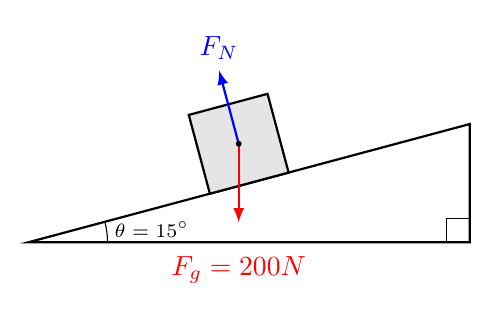
\begin{tikzpicture}
            \draw[thick, black] (0,0) -- (5.6, 0) -- (5.6, 1.5) -- cycle;
            \draw[] (5.3, 0) -- (5.3, 0.3) -- (5.6, 0.3);
            \draw[] (1, 0) arc (0:15:1) node[right, font = \scriptsize, yshift = -0.1cm] 
            	{$\theta = 15^{\circ}$};
            \draw[thick, black, fill=gray!20] (2.3, 0.616) -- (3.3, 0.884) -- 
            	(3.032, 1.884) -- (2.032, 1.616) -- cycle;
            \draw[-latex, thick, blue] (2.666, 1.25) -- (2.416, 2.183) 
            	node[above] {$F_N$};
            \draw[-latex, thick, red] (2.666, 1.25) -- (2.666, 0.25) 
            	node[below, yshift = -0.3cm] {$F_g = 200\text{ N}$};
            \draw[black, fill=black] (2.666, 1.25) circle (0.03cm);
	\end{tikzpicture}
\end{center}

Notice that the normal force is perpendicular to the ramp! We want to know how 
much force it takes to push the load up the ramp, so we will ``split" the 
weight force vector into two parts: one part parallel to the ramp ($F_{g,\vert 
\vert}$) and one part perpendicular ($F_{g, \perp}$):

\begin{center}
	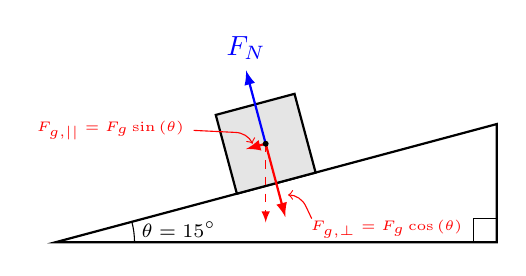
\begin{tikzpicture}
            \draw[thick, black] (0,0) -- (5.6, 0) -- (5.6, 1.5) -- cycle;
            \draw[] (5.3, 0) -- (5.3, 0.3) -- (5.6, 0.3);
            \draw[] (1, 0) arc (0:15:1) 
            	node[right, font = \scriptsize, yshift = -0.1cm] 
            	{$\theta = 15^{\circ}$};
            \draw[thick, black, fill=gray!20] (2.3, 0.616) -- (3.3, 0.884) -- 
            	(3.032, 1.884) -- (2.032, 1.616) -- cycle;
            \draw[-latex, thick, blue] (2.666, 1.25) -- (2.416, 2.183) 
            	node[above] {$F_N$};
            \draw[-latex, thin, red, dashed] (2.666, 1.25) -- (2.666, 0.25);
            \draw[-latex, thick, red] (2.666, 1.25) -- (2.916, 0.317);
            \draw[-latex, thick, red] (2.666, 1.25) -- (2.416, 1.183);
            \draw[black, fill=black] (2.666, 1.25) circle (0.03cm);
            \draw[red, <-, thin] (2.95, 0.6) arc (90:25:0.25) -- (3.25, 0.3) 
            	node[below, font = \tiny, xshift = 0.95cm, yshift = 0.1cm] 
            	{$F_{g,\perp} = F_g \cos{\left( \theta \right)}$};
            \draw[red, <-, thin] (2.5, 1.25) arc (25:90:0.25) -- (1.75, 1.42) 
            	node[left, font = \tiny] 
            	{$F_{g,\vert \vert} = F_g \sin{ \left( \theta \right)}$};
	\end{tikzpicture}
\end{center}

We did this by treating the weight vector as the hypotenuse of a right triangle 
with legs perpendicular and parallel to the ramp. You'll learn how to do this 
and why it works in the chapter on vectors. For now, just trust that the part 
of the hand trolley's weight that is perpendicular to the ramp is $F_g \cos{ 
\left( \theta \right) }$ and the part that is parallel to the ramp is $F_g 
\sin{ \left( \theta \right) }$.

What force do you need to overcome to push the hand trolley up the ramp? Just 
the part of the weight that is parallel to the ramp! You'll need to apply an 
equal force in the opposite direction (up the ramp) to move the hand trolley:

\begin{center}
	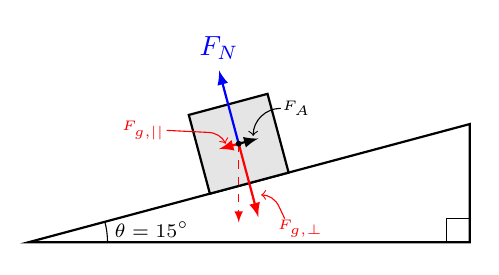
\begin{tikzpicture}
            \draw[thick, black] (0,0) -- (5.6, 0) -- (5.6, 1.5) -- cycle;
            \draw[] (5.3, 0) -- (5.3, 0.3) -- (5.6, 0.3);
            \draw[] (1, 0) arc (0:15:1) 
            	node[right, font = \scriptsize, yshift = -0.1cm] 
            	{$\theta = 15^{\circ}$};
            \draw[thick, black, fill=gray!20] (2.3, 0.616) -- (3.3, 0.884) -- 
            	(3.032, 1.884) -- (2.032, 1.616) -- cycle;
            \draw[-latex, thick, blue] (2.666, 1.25) -- (2.416, 2.183) 
            	node[above] {$F_N$};
            \draw[-latex, thin, red, dashed] (2.666, 1.25) -- (2.666, 0.25);
            \draw[-latex, thick, red] (2.666, 1.25) -- (2.916, 0.317);
            \draw[-latex, thick, red] (2.666, 1.25) -- (2.416, 1.183);
            \draw[red, <-, thin] (2.95, 0.6) arc (90:25:0.25) -- (3.25, 0.3) 
            	node[below, font = \tiny, xshift = 0.2cm, yshift = 0.1cm] 
            	{$F_{g,\perp}$};
            \draw[red, <-, thin] (2.5, 1.25) arc (25:90:0.25) -- (1.75, 1.42) 
            	node[left, font = \tiny, xshift = 0.1cm] 
            	{$F_{g,\vert \vert}$};
            \draw[thick, black, -latex] (2.666, 1.25) -- (2.916, 1.317);
            \draw[thin, black, <-] (2.85, 1.35) arc (180:90:0.35) 
            	node[right, font = \tiny, xshift = -0.1cm] {$F_A$};
            \draw[black, fill=black] (2.666, 1.25) circle (0.03cm);
	\end{tikzpicture}
\end{center}

So, we know that you are pushing with an applied force of $F_A = F_{g, \vert 
\vert} = F_{g} \sin{ \left( \theta \right) }$. Therefore, the work you would do 
pushing the hand trolley up the ramp is:
$$F_A \cdot L = F_{g} \sin{ \left( \theta \right)} \cdot \left( \frac{V}{\sin{ 
\left( \theta \right)}} \right) = F_{g} \cdot V = 300 \text{ }J$$

Therefore, when using a ramp, you still perform the same amount of work! This 
is a key property of simple machines: \textit{the work done doesn't change}.

So what makes it ``easier" to use a ramp to lift the hand trolley? The fact 
that you need to apply less \textit{force} to move the hand trolley ($F_A < 
F_g$). Now, let's look at the mechanical advantage of the ramp. In this case, 
the mechanical advantage is given by:
$$MA = \frac{F_g}{F_A}$$

Substituting for $F_A$, we see that:
$$MA = \frac{F_g}{F_g \sin{ \left( \theta \right)}} = \frac{1}{\frac{V}{L}} 
= \frac{L}{V}$$

So for a ramp whose length is $L$ and vertical rise is $V$, the mechanical 
advantage is equal to the length divided by the rise. 

\begin{mdframed}[style = important, frametitle={Ramps}]
For a ramp, the mechanical advantage is equal to $\frac{L}{V}$ and the force 
needed to push an object with weight $W$ up the ramp is given by $W \cdot 
\frac{V}{L} = W \cdot \sin{ \left( \theta \right)}$, where $L$ is the length 
of the ramp, $V$ is the vertical rise of the ramp, and $\theta$ is the angle 
the ramp forms with the (horizontal) ground.
\end{mdframed}

\begin{Exercise}[title={Ramp}, label=ramp]
You need to lift a barrel of oil with a mass of 136 kilograms. You can apply a 
force of up to 300 newtons. You need to get the barrel onto a platform that is 
2 meters high. What is the shortest length of inclined plane you can use?
\end{Exercise}
\begin{Answer}[ref=ramp]
The weight of the barrel is \( 136 \text{ kg} \times 9.8 \text{ } 
\frac{\text{m}}{\text{s}^2}= 1332.8 \text{ N}\).

Let \( L \) be the length of the inclined plane. The force needed to push the 
barrel up is related by:

\[
300 \text{ N}= \frac{2 \text{ m}}{L} \times 1332.8 \text{ N}
\]

Solving for \( L \), we find \( L = \frac{2 \text{ m} \times 1332.8}{300} 
\approx 8.885 \text{ m}\).
\end{Answer}

\section{Levers}

A lever pivots on a fulcrum. To decrease the necessary force, the load is placed 
closer to the fulcrum than where the force is applied.

Physicists also discuss the concept of \newterm{torque} created by a force. When 
you apply force to a lever, the torque is the product of the force you exert and 
the distance from the point of rotation.

Torque is typically measured in newton-meters (N$\cdot$m).

To balance two torques, the products of force and distance must be equal. Thus, 
assuming the forces are applied in the correct direction, the equation becomes:

\[
R_L F_g = R_A F_A
\]

where \( R_L \) and \( R_A \) represent the distances from the fulcrum to where 
the load’s weight and the applied force are exerted, respectively, and \( F_g \) 
and \( F_A \) are the magnitudes of the forces.

%image showing lever with everything labeled

\begin{Exercise}[title={Lever}, label=lever]
Paul, whose mass is 70 kilograms, sits on a see-saw 4 meters from the fulcrum. 
Jan, whose mass is 50 kilograms, wishes to balance the see-saw. How far should 
Jan sit from the fulcrum?

\begin{center}
\includegraphics[width=0.6\textwidth]{seesaw.png}
\end{center}

\end{Exercise}
\begin{Answer}[ref=lever]
Paul exerts a force of \( 70 \text{ kg} \times 9.8 \text{ } \frac{\text{m}}{
\text{s}^2} = 686 \text{ N}\) at a distance of 4 meters from the fulcrum, 
creating a torque of \( 686 \text{ N}\times 4 \text{ m} = 2744 \text{ N} \cdot 
\text{m} \). Jan exerts a force of \( 50 \text{ kg} \times 9.8 \text{ } \frac{
\text{m}}{\text{s}^2}= 490 \text{ N}\).

Let \( r \) be the distance from the fulcrum to Jan's seat. To balance the torques:

\[
490 \text{ N}\times r = 2744 \text{ N} \cdot \text{m}
\]

Solving for \( r \), we find \( r = \frac{2744}{490} \approx 5.6 \) meters.
\end{Answer}

\section{Gears}

Gears have teeth that mesh with each other. When you apply torque to one gear, 
it transfers torque to the other. The resulting torque is increased or decreased 
depending on the ratio of the number of teeth on the gears. 
%explain connection between teeth and radius
%example for torque vs power: riding your bike up a hill, gears in your car

\includegraphics[width=0.7\textwidth]{gearsNew.png}

If \( N_A \) is the number of teeth on the gear you are turning with a torque of 
\( T_A \), and \( N_L \) is the number of teeth on the gear it is turning, the r
esulting torque is:

\[
T_L = \frac{N_A}{N_L} T_A
\]
% maybe add more on this? not sure how important it is or if it needs to be emphasized more
\begin{Exercise}[title={Gears}, label=gear]
In a bicycle, the goal is not always to gain mechanical advantage, but to spin 
the pedals slower while applying more force.

You like to pedal your bike at 70 revolutions per minute. The chainring 
connected to your pedals has 53 teeth. The circumference of your tire is 2.2 
meters. You want to ride at 583 meters per minute.

How many teeth should the rear sprocket have?
\end{Exercise}
\begin{Answer}[ref=gear]
The equation relating these quantities is:

\[
583 = 70 \times 2.2 \times \frac{53}{n}
\]

Solving for \( n \), we find \( n = 14 \) teeth.
\end{Answer}

\section{Hydraulics}

In a hydraulic system, such as a car's braking system, you exert force on a 
piston filled with fluid. The fluid transmits this pressure into another 
cylinder, where it pushes yet another piston that moves the load. The pressure 
at each end of the hydraulic system must be the same. 

\includegraphics[width=\textwidth]{hydraulicsNew.png}

\newterm{Pressure} is force applied to an area; it is calculated by dividing 
the force by the area.  The pressure in the fluid is typically measured in 
pascals (Pa), which is equivalent to \(N / m^2\). We will use pascals for this 
calculation.

To calculate the pressure you create, divide the force applied $F_{a}$ by the 
area of the piston head $A$. To determine the force on the other piston, 
multiply the pressure by the area of the second piston.
% added equation for pressure
\[
P = \frac{F_{a_1}}{A_1} = \frac{F_{a_2}}{A_2}
\]


\begin{Exercise}[title={Hydraulics}, label=hydraulics]
Your car has disc brakes. When you apply 2,500,000 pascals of pressure to the 
brake fluid, the car stops quickly. As the car designer, you want this to 
require only 12 newtons of force from the driver's foot.

What should the radius of the master cylinder (the piston the driver pushes) be?
\end{Exercise}
\begin{Answer}[ref=hydraulics]
We are solving for the radius \( r \) of the piston. The area of the piston is 
\( \pi r^2 \), so the pressure is:

\[
\text{Pressure} = \frac{12}{\pi r^2}
\]

Setting the pressure equal to 2,500,000 pascals:

\[
2,500,000 = \frac{12}{\pi r^2}
\]

Solving for \( r \), we find:

\[
r = \sqrt{\frac{12}{\pi \times 2.5 \times 10^6}} \approx 0.00124 \text{ meters}.
\]
\end{Answer}

\section{Pulleys}

\section{Wedges}
